\subsubsection{Забудем на время о MSVC}

\ac{SEH} в Windows предназначен для обработки исключений, тем не менее, с \Cpp и \ac{OOP} он никак не связан.
Здесь мы рассмотрим \ac{SEH} изолированно от Си++ и расширений MSVC.

\myindex{Windows!TIB}
\myindex{Windows!Win32!RaiseException()}
Каждый процесс имеет цепочку \ac{SEH}-обработчиков, и адрес последнего записан в \ac{TIB}.
Когда происходит исключение (деление на ноль, обращение по неверному адресу в памяти, 
пользовательское исключение, поднятое при помощи \TT{RaiseException()}),
\ac{OS} находит последний обработчик в \ac{TIB} и вызывает его, 
передав ему информацию о состоянии \ac{CPU} в момент исключения
(все значения регистров, итд.).
Обработчик выясняет, то ли это исключение, для которого он создавался?

Если да, то он обрабатывает исключение.
Если нет, то показывает \ac{OS} что он не может его обработать и \ac{OS} вызывает следующий обработчик
в цепочке, и так до тех пор, пока не найдется обработчик способный обработать исключение.

В самом конце цепочки находится стандартный обработчик, показывающий всем очень известное окно, 
сообщающее что процесс упал, 
сообщает также состояние \ac{CPU} в момент падения и позволяет собрать и отправить информацию обработчикам 
в Microsoft. 

\begin{figure}[H]
\centering
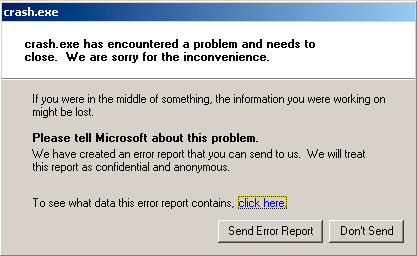
\includegraphics[width=0.6\textwidth]{OS/SEH/1/crash_xp1.png}
\caption{Windows XP}
\end{figure}

\begin{figure}[H]
\centering
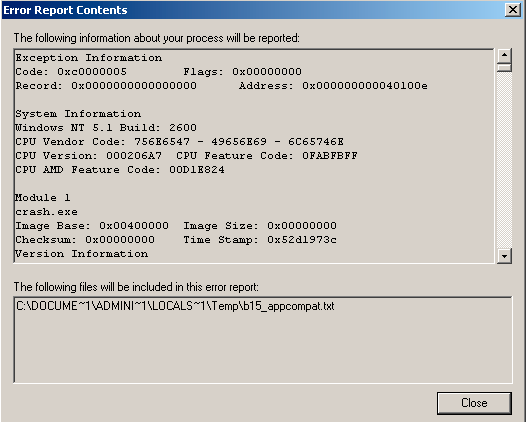
\includegraphics[width=0.6\textwidth]{OS/SEH/1/crash_xp2.png}
\caption{Windows XP}
\end{figure}

\begin{figure}[H]
\centering
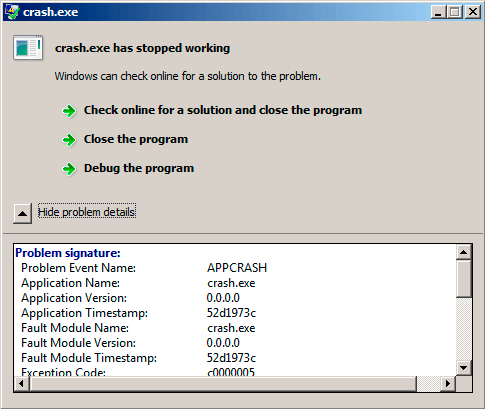
\includegraphics[width=0.6\textwidth]{OS/SEH/1/crash_win7.png}
\caption{Windows 7}
\end{figure}

\begin{figure}[H]
\centering
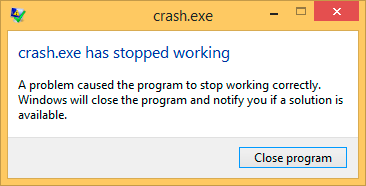
\includegraphics[width=0.6\textwidth]{OS/SEH/1/crash_win81.png}
\caption{Windows 8.1}
\end{figure}

Раньше этот обработчик назывался Dr. Watson
\footnote{\href{http://go.yurichev.com/17046}{wikipedia}}.

Кстати, некоторые разработчики делают свой собственный обработчик,
отправляющий информацию о падении программы им самим.\\
\myindex{Windows!Win32!SetUnhandledExceptionFilter()}
Он регистрируется при помощи функции \TT{SetUnhandledExceptionFilter()} 
и будет вызван если \ac{OS} не знает как иначе обработать исключение.

\myindex{\oracle}
А, например, \oracle в этом случае генерирует огромные дампы, 
содержащие всю возможную информацию и состоянии \ac{CPU} и памяти.

Попробуем написать свой примитивный обработчик исключений.
Этот пример основан на примере из \PietrekSEH.
Он должен компилироваться с опцией SAFESEH: \TT{cl seh1.cpp /link /safeseh:no}.
Подробнее об опции SAFESEH здесь: \href{http://go.yurichev.com/17252}{MSDN}.
	
\lstinputlisting{OS/SEH/1/1.cpp}

Сегментный регистр FS: в win32 указывает на \ac{TIB}.
Самый первый элемент \ac{TIB} это указатель на последний обработчик в цепочке.
Мы сохраняем его в стеке и записываем туда адрес своего обработчика.
Эта структура называется \TT{\_EXCEPTION\_REGISTRATION}, 
это простейший односвязный список, и эти элементы хранятся прямо в стеке.

\begin{lstlisting}[caption=MSVC/VC/crt/src/exsup.inc]
\_EXCEPTION\_REGISTRATION struc
     prev    dd      ?
     handler dd      ?
\_EXCEPTION\_REGISTRATION ends
\end{lstlisting}

Так что каждое поле \q{handler} указывает на обработчик,
а каждое поле \q{prev} указывает на предыдущую структуру в стеке.
Самая последняя структура имеет \TT{0xFFFFFFFF} (-1) в поле \q{prev}.

\begin{center}
\ifdefined\ebook
\begin{tikzpicture}[thick,scale=0.50, every node/.style={scale=0.50}]
\else
\begin{tikzpicture}[thick,scale=0.85, every node/.style={scale=0.85}]
\fi
	\tikzstyle{every path}=[thick]
	\tikzstyle{undefined}=[draw,rectangle,minimum height=1cm, minimum width=3.5cm, text width=3.5cm]
	\tikzstyle{node}=[draw,rectangle,minimum height=1cm, minimum width=3.5cm, text width=3.5cm, fill=gray!20]
	
	\node[node] (fs) [minimum width=1.5cm, text width=1.5cm] {FS:0};

	\node[node] (tib1) [right=1.5cm of fs] {+0: \_\_except\_list};
	\node[undefined] (tib2) [below of=tib1] {+4: \dots};
	\node[undefined] (tib3) [below of=tib2] {+8: \dots};
	\node (tib_text) [above of=tib1] {TIB};
	
	\draw [->] (fs.east) -- (tib1.west);

	\node[undefined] (u1) [text centered, right=2.5cm of tib1] {\dots};
	\node [node] (n1prev) [below of=u1] {Prev=0xFFFFFFFF};
	\node [node] (n1handler) [below of=n1prev] {Handle};
	\node [node] (n1handler_text) [right=1cm of n1handler] {\HandlerFunction};
	\draw [->] (n1handler.east) -- (n1handler_text.west);
	\node[undefined] (u2) [text centered, below of=n1handler] {\dots};
	\node [node] (n2prev) [below of=u2] {Prev};
	\node [node] (n2handler) [below of=n2prev] {Handle};
	\node [node] (n2handler_text) [right=1cm of n2handler] {\HandlerFunction};
	\draw [->] (n2handler.east) -- (n2handler_text.west);
	\node[undefined] (u3) [text centered, below of=n2handler] {\dots};
	\node [node] (n3prev) [below of=u3] {Prev};

	\node [node] (n3handler) [below of=n3prev] {Handle};
	\node [node] (n3handler_text) [right=1cm of n3handler] {\HandlerFunction};
	\draw [->] (n3handler.east) -- (n3handler_text.west);
	\node[undefined] (u4) [text centered, below of=n3handler] {\dots};
	\node (stack_text) [above of=u1] {\IFRU{Стек}{Stack}};
	
	\node (n2block_pt1) [inner sep=0pt, above left=0cm and 0cm of n2prev] {};
	\node (n2block_pt2) [inner sep=0pt, above left=0cm and 0.5cm of n2prev] {};
	\draw [->] (n3prev.west) .. controls +(left:0.5cm) and (n2block_pt2) .. (n2block_pt1);

	\node (n1block_pt1) [inner sep=0pt, above left=0cm and 0cm of n1prev] {};
	\node (n1block_pt2) [inner sep=0pt, above left=0cm and 0.8cm of n1prev] {};
	\draw [->] (n2prev.west) .. controls +(left:0.8cm) and (n1block_pt2) .. (n1block_pt1);
	
	\node (n3block_pt1) [inner sep=0pt, above left=0cm and 0cm of n3prev] {};
	\node (n3block_pt2) [inner sep=0pt, above left=0cm and 1.25cm of n3prev] {};
	\draw [->] (tib1.east) .. controls +(right:1.25cm) and (n3block_pt2) .. (n3block_pt1);


\end{tikzpicture}
\end{center}


После инсталляции своего обработчика, вызываем \TT{RaiseException()}\footnote{\href{http://go.yurichev.com/17253}{MSDN}}.
Это пользовательские исключения. 
Обработчик проверяет код.\\
Если код \TT{0xE1223344}, то он возвращает \TT{ExceptionContinueExecution},
что сигнализирует системе что обработчик скорректировал состояние CPU (обычно это регистры EIP/ESP) и что \ac{OS} может
возобновить исполнение треда.
Если вы немного измените код так что обработчик будет возвращать \TT{ExceptionContinueSearch},
то \ac{OS} будет вызывать остальные
обработчики в цепочке, и вряд ли найдется тот, кто обработает ваше исключение,
ведь информации о нем (вернее, его коде) ни у кого нет.
Вы увидите стандартное окно Windows о падении процесса.

Какова разница между системными исключениями и пользовательскими? Вот системные:

\small
\begin{center}
\begin{tabular}{ | l | l | l | }
\hline
\HeaderColor как определен в WinBase.h & 
\HeaderColor как определен в ntstatus.h & 
\HeaderColor численное значение \\
\hline
EXCEPTION\_ACCESS\_VIOLATION          & STATUS\_ACCESS\_VIOLATION           & 0xC0000005 \\
\hline
EXCEPTION\_DATATYPE\_MISALIGNMENT     & STATUS\_DATATYPE\_MISALIGNMENT      & 0x80000002 \\
\hline
EXCEPTION\_BREAKPOINT                & STATUS\_BREAKPOINT                 & 0x80000003 \\
\hline
EXCEPTION\_SINGLE\_STEP               & STATUS\_SINGLE\_STEP                & 0x80000004 \\
\hline
EXCEPTION\_ARRAY\_BOUNDS\_EXCEEDED     & STATUS\_ARRAY\_BOUNDS\_EXCEEDED      & 0xC000008C \\
\hline
EXCEPTION\_FLT\_DENORMAL\_OPERAND      & STATUS\_FLOAT\_DENORMAL\_OPERAND     & 0xC000008D \\
\hline
EXCEPTION\_FLT\_DIVIDE\_BY\_ZERO        & STATUS\_FLOAT\_DIVIDE\_BY\_ZERO       & 0xC000008E \\
\hline
EXCEPTION\_FLT\_INEXACT\_RESULT        & STATUS\_FLOAT\_INEXACT\_RESULT       & 0xC000008F \\
\hline
EXCEPTION\_FLT\_INVALID\_OPERATION     & STATUS\_FLOAT\_INVALID\_OPERATION    & 0xC0000090 \\
\hline
EXCEPTION\_FLT\_OVERFLOW              & STATUS\_FLOAT\_OVERFLOW             & 0xC0000091 \\
\hline
EXCEPTION\_FLT\_STACK\_CHECK           & STATUS\_FLOAT\_STACK\_CHECK          & 0xC0000092 \\
\hline
EXCEPTION\_FLT\_UNDERFLOW             & STATUS\_FLOAT\_UNDERFLOW            & 0xC0000093 \\
\hline
EXCEPTION\_INT\_DIVIDE\_BY\_ZERO        & STATUS\_INTEGER\_DIVIDE\_BY\_ZERO     & 0xC0000094 \\
\hline
EXCEPTION\_INT\_OVERFLOW              & STATUS\_INTEGER\_OVERFLOW           & 0xC0000095 \\
\hline
EXCEPTION\_PRIV\_INSTRUCTION          & STATUS\_PRIVILEGED\_INSTRUCTION     & 0xC0000096 \\
\hline
EXCEPTION\_IN\_PAGE\_ERROR             & STATUS\_IN\_PAGE\_ERROR              & 0xC0000006 \\
\hline
EXCEPTION\_ILLEGAL\_INSTRUCTION       & STATUS\_ILLEGAL\_INSTRUCTION        & 0xC000001D \\
\hline
EXCEPTION\_NONCONTINUABLE\_EXCEPTION  & STATUS\_NONCONTINUABLE\_EXCEPTION   & 0xC0000025 \\
\hline
EXCEPTION\_STACK\_OVERFLOW            & STATUS\_STACK\_OVERFLOW             & 0xC00000FD \\
\hline
EXCEPTION\_INVALID\_DISPOSITION       & STATUS\_INVALID\_DISPOSITION        & 0xC0000026 \\
\hline
EXCEPTION\_GUARD\_PAGE                & STATUS\_GUARD\_PAGE\_VIOLATION       & 0x80000001 \\
\hline
EXCEPTION\_INVALID\_HANDLE            & STATUS\_INVALID\_HANDLE             & 0xC0000008 \\
\hline
EXCEPTION\_POSSIBLE\_DEADLOCK         & STATUS\_POSSIBLE\_DEADLOCK          & 0xC0000194 \\
\hline
CONTROL\_C\_EXIT                      & STATUS\_CONTROL\_C\_EXIT             & 0xC000013A \\
\hline
\end{tabular}
\end{center}
\normalsize

Так определяется код:

\begin{center}
\begin{bytefield}[bitwidth=0.03\linewidth]{32}
\bitheader[endianness=big]{31,29,28,27,16,15,0} \\
\bitbox{2}{S} & 
\bitbox{1}{U} &
\bitbox{1}{0} & 
\bitbox{12}{Facility code} &
\bitbox{16}{Error code}
\end{bytefield}
\end{center}

S это код статуса: 
11 --- ошибка;
10 --- предупреждение;
01 --- информация;
00 --- успех.
U ---- является ли этот код пользовательским, а не системным.

Вот почему мы выбрали 0xE1223344 --- E\textsubscript{16} (1110\textsubscript{2}) 0xE (1110b)
означает что это 1) пользовательское исключение; 2) ошибка.
Хотя, если быть честным, этот пример нормально работает и без этих старших бит.

Далее мы пытаемся прочитать значение из памяти по адресу 0.
Конечно, в win32 по этому адресу обычно ничего нет, и сработает исключение.
Однако, первый обработчик, который будет заниматься этим делом\EMDASH{}ваш, и он узнает об этом
первым, проверяя код на соответствие с константной \TT{EXCEPTION\_ACCESS\_VIOLATION}.

А если заглянуть в то что получилось на ассемблере,
то можно увидеть, что код читающий из памяти по адресу 0, выглядит так:

\lstinputlisting[caption=MSVC 2010]{OS/SEH/1/1_fragment.asm}

Возможно ли \q{на лету} исправить ошибку и предложить программе исполняться далее?
Да, наш обработчик может изменить значение в \EAX и предложить \ac{OS} исполнить эту же инструкцию еще раз.
Что мы и делаем. \printf напечатает 1234, потому что после работы нашего обработчика, \EAX будет не 0,
а будет содержать адрес глобальной переменной \TT{new\_value}.
Программа будет исполняться далее.

Собственно, вот что происходит: срабатывает защита менеджера памяти в \ac{CPU}, 
он останавливает работу треда, отыскивает в ядре Windows обработчик исключений, 
тот, в свою очередь, начинает вызывать обработчики из цепочки \ac{SEH}, по одному.

Мы компилируем это всё в MSVC 2010, но конечно же, нет никакой гарантии 
что для указателя будет использован именно регистр \EAX.

Этот трюк с подменой адреса эффектно выглядит, и мы рассматриваем его здесь для наглядной иллюстрации работы \ac{SEH}.

Тем не менее, трудно припомнить, применяется ли где-то подобное на практике для исправления ошибок \q{на лету}.

Почему SEH-записи хранятся именно в стеке а не в каком-то другом месте?
Возможно, потому что \ac{OS} не нужно заботиться об освобождении этой информации, эти записи
просто пропадают как ненужные когда функция заканчивает работу.

\myindex{\CStandardLibrary!alloca()}
Это чем-то похоже на alloca(): (\myref{alloca}).

